\documentclass[10pt, conference, compsocconf]{IEEEtran}
\hyphenation{op-tical net-works semi-conduc-tor}
\usepackage{amsmath}
\usepackage{algorithm}
\usepackage{algorithmic}
\usepackage{color}
\usepackage{supertabular,booktabs}
\usepackage{graphicx}
\usepackage{bm}
\usepackage[colorlinks,linkcolor=red,anchorcolor=blue,citecolor=green,CJKbookmarks=True]{hyperref}
\begin{document}
\title{Analysis of high frequency stock data based on machine learning}
\author
{\IEEEauthorblockN{Xiaoyang Wu \IEEEauthorrefmark{1}\IEEEauthorrefmark{2},Jiahui Wu\IEEEauthorrefmark{1}\IEEEauthorrefmark{2},Zheng Xie\IEEEauthorrefmark{1}\IEEEauthorrefmark{2}, JinYuan Yu\IEEEauthorrefmark{1}\IEEEauthorrefmark{2}
}
\IEEEauthorblockA
{
	\IEEEauthorrefmark{1}Likelihood Technology\\
}
\IEEEauthorblockA
{
	\IEEEauthorrefmark{2}Sun Yat-sen University\\
}
$ $\\
$\{wuxy65,wujh56,xiezh25,yujy25\}@mail2.sysu.edu.cn$
}
\maketitle
\begin{abstract}
In recent years, few studies have been published in the field of high frequency financial data analysis, since such findings can be directly 
utilized to make profits. In this under-explored field, we hope to discover some hidden patterns in the stock market of Mainland China by 
analyzing tick-level financial data drawn from Shanghai Stock Exchange. Since the size of tick-level data is tremendously large, machine 
learning methods are the ideal analytic tools due to their reputations of finding latent patterns in big data. In the experiments, we achieved 
high prediction performances using Long Short-term Memory Recurrent Neural Network and other two tree-based algorithms (Random Forest and 
XGBoost) independently with sophisticated financial feature engineering. We can predict the trends of tick-level data and 2.5 minutes-level 
data with accuracy of  92\% and 74\% respectively, which provide strong investment guidance in real time trading. 
\end{abstract}

\begin{IEEEkeywords}
High Frequency Stock Data;Machine Learning;LSTM;XGBoost;Random Forest;Feature Importance;
\end{IEEEkeywords}

\IEEEpeerreviewmaketitle

\section{INTRODUCTION}
It is commonly acknowledged that prices in stock market are the most difficult and mysterious time series to predict though we all admit that 
there should be some ‘universal’ laws directing the fluctuation of consecutive prices. 
Large number of experiments have been conducted to model daily price fluctuation in stock market whereas few study can be seen in deciphering 
the code in high frequency data. Having tick-level time series data from Shanghai Stock Exchange (data presented in forms of every three to 
five seconds, including current price, buy side volume and many other basic features) in hand, we mainly want to discover temporal correlation 
between prices of consecutive or close tick and features with strong prediction power as well as high interpretability.
In this paper, we respectively employ traditional machine learning methods, such as Random Forest and XGBoost, in comparison with deep learning 
method Long Short-term Memory Recurrent Neural Network in terms of their prediction power within high frequency environment, Based on tick-level 
time series data from Shanghai Stock Exchange, we focus on trend prediction on price of next tick as well as mean price of 2.5 minutes ahead, 
the latter of which is an average of stock price within the range of five minutes starting from current tick. Considering large proportion of 
unchanged price in the next tick, We propose two evaluation criteria in defining prediction accuracy, the first of which is ignoring unchanged 
price and only check whether the trend prediction is correct when real price does fluctuate. The other is assuming the existence of price lag, 
that is to say, we do not judge immediately when the predicted trend tells a rise or a fall whereas price remain unchanged in the next tick, 
instead, it is the first fluctuation in price since current tick that is captured to evaluate whether the prediction is right or wrong. The 
underlying intuition is that the driven force for price to rise or fall might not reach a threshold during such a tiny time step for price to 
react, thus we should allow for hysteretic price change.
Experiments with real data from SSE show that LSTM slightly outperform both Random Forest and XGBoost in terms of trend prediction of next-tick 
price with an accuracy up to 0.925 using first criterion and 0.83 using the other, reflecting a long or short term price dependency with 
historical data. LSTM still ranks top among other methods in predicting relatively further future information (mean price of 2.5min ahead), 
with an accuracy up to 0.741 under first criterion, in which the sharp decline is mainly due to more uncontrollable noises within this time 
range. The paper is organized as follows: Section 2 briefly introduces the mechanisms of models and methods that we use in our project, 
including LSTM, Random Forests and XGBoost. Section 3 presents the procedure of our experiments as well as the performance of different methods. 
In the last section, we discusses a few findings in high frequency environment and proposes some other directions for future improvement. 

\vspace{0.5cm}

\section{METHODS}
\subsection{LSTM}
The Recurrent Neural Network (RNN) is an extremely powerful model for problems in machine learning that require identifying complex dependencies 
between temporally distant inputs. Due to its special architecture which contains information of historic input, It has been found to be not 
only very good at predicting next character in the text or the next word in a sequence, but also inspiring in some complex tasks. Though 
powerful, training them has proved to be problematic because the back propagated gradients either grow or shrink at each time step, so over 
many time steps, they typically explode or vanish. Besides this, theoretical and empirical evidence shows that it is difficult for RNNs to 
learn to restore information for very long which is another obstacle for network to discover and learn relatively long-term dependencies.\\

\begin{figure}[ht]
	\centering
	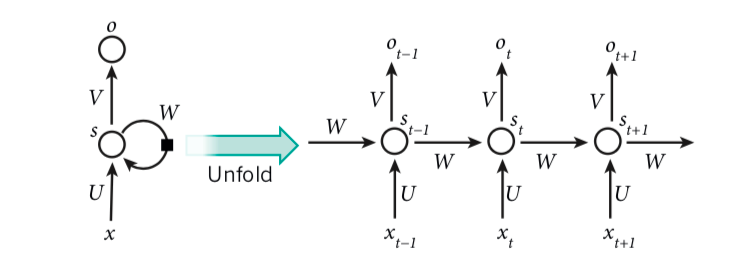
\includegraphics[scale=0.5]{1.png}
	\caption{cycle in RNN} \label{fig 1}
\end{figure}

Those experimental problems directly gave birth to several specifically-designed RNN with explicit memory. Among those, Long Short-term Memory 
Network is most widely used. With the help of a special unit called memory cell which acts like an accumulator or a gated leaky neuron, its 
real-valued state can be copied via a connection to itself with a weight of one. However, this self-connection is multiplicatively gated by 
another unit that learns to decide when to clear the content of the memory.\\

\begin{figure}[ht]
	\centering
	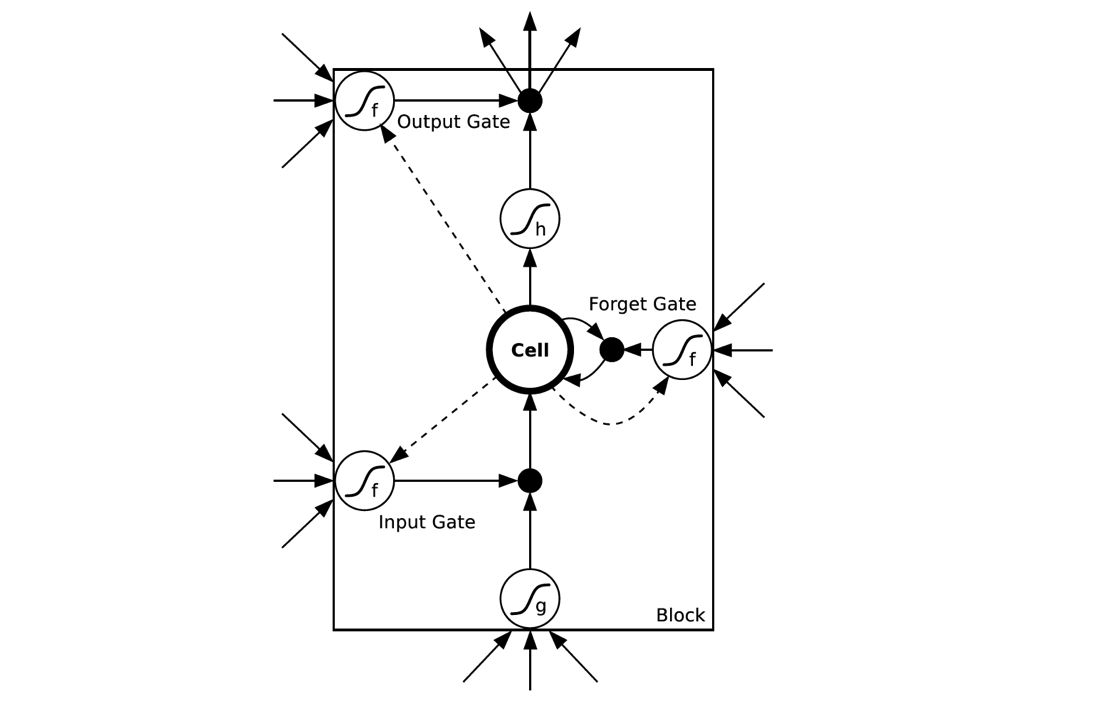
\includegraphics[scale=0.3]{2.png}
	\caption{cell} \label{fig 2}
\end{figure}

\subsection{Random Forest}
Random Forests is an ensemble learning method mainly used for classification and regression problems. As can be learned from the name, it is 
constructed based on a multitude of decision trees which are trained on differently-sampled training data and adopt differently-sampled features. \\
In comparison with traditional single decision tree which is subject to overfitting when there are many features and trees are grown deep, 
Random Forests average the variance through integrating results of multiple deep decision trees, each constructed on sub-set of total features 
and trained on different parts of the same training set. It is a tradeoff between variance and bias, generally, Random Forests comes at an expense of a small increase in the 
model bias but can greatly boost the performance in the final model, especially its generalization power.\\

\begin{figure}[ht]
	\centering
	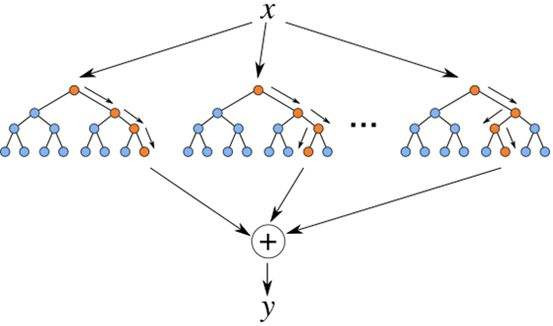
\includegraphics[scale=0.5]{3.png}
	\caption{Random Forest} \label{fig 3}
\end{figure}

\subsection{XGBoost}
XGBoost is an optimized distributed gradient boosting system designed to be highly efficient, flexible and portable. It implements machine learning algorithms under the Gradient Boosting framework. \\
Specifically, XGBoost is a tree ensemble model. Unlikely Random Forest where trees are independent of each other, there is a series of trees in XGBoost and the output of one tree will influence the training process of the following 
trees. Note that the final prediction for a given example is the sum of predictions from each tree.\\
The great merit of XGBoost is its scalability in all scenarios. The system runs more than ten times faster than existing popular solutions on a single machine and scales to billions of examples in distributed or memory-limited settings.\\

\section{EXPERIMENT}
\subsection{Construction of dataset}
\begin{enumerate}
	\item Introduction to tick data in Chinese stock market\\
	There are only two stock exchange in Mainland China, namely, Shanghai Stock Exchange and Shenzhen Stock Exchange. During trading time, both of them release a snapshot of the stock market every 3 to 5 seconds( only if there is a new
	 deal; otherwise, no new information will be released), including the price of the last deal during the period and the latest version of the double auction book. Such a snapshot constitutes one piece of tick data. 
	\item Stock selection\\
	We simply choose three constituent stocks of CSI300 which fluctuate rationally and do not have an explosive growth or collapse during the period we carry out our research. The  reason is that if there is an explosive growth or collapse, 
	a machine learning algorithm can learn the trend more easily.
	\item Time span of the data\\
	The environment of the whole market change all the time, which means that the relation between known data and future price changes as time goes on. Consequently, we use only five trading days’ tick data (from June 15th, 2018 to June
	22th, 2018) of the three stocks and assume that the environment is the same during this period.
	\item Features\\
	For each piece of tick data (released every 3 to 5 seconds), we have some features obtained from the exchange. Apart from these, we also construct some new features in order to improve the performance of our machine learning models. 
	Now we are going to explain each of them in detail.\\
	(1) price\\
	The latest price during the period.

	(2) vol\\
	The total trading volume during the period.

	(3) amount\\
	$$
		amount = price \cdot vol 
	$$

	(4) buy1, buy2, buy3, buy4, buy5\\
	The highest five price levels at which some traders are willing to buy a particular stock. Note that buy1 $>$ buy2 $>$ buy3 $>$ buy4 $>$ buy5. 

	(5) bc1, bc2, bc3, bc4, bc5\\
	The volumes corresponding to the five price levels (buy1, buy2, buy3, buy4, buy5).

	(6) sale1, sale2, sale3, sale4, sale5\\
	The lowest five price levels at which some traders are willing to sell a particular stock. Note that sale1 $<$ sale2 $<$ sale3 $<$ sale4 $<$ sale5. 

	(7) sc1, sc2, sc3, sc4, sc5\\
	The volumes corresponding to the five price levels(sale1, sale2, sale3, sale4, sale5).

	(8) w\_buy\\
	$$
		w\_buy = bc1 + bc2 + bc3 + bc4 + bc5
	$$

	(9) w\_sale\\
	$$
		w\_sale = sc1 + sc2 + sc3 + sc4 + sc5
	$$

	(10) wb\\
	$$
		wb = \frac{w\_buy}{w\_sale}
	$$

	(11) lb
	$$
		lb = \frac{(\sum_{i=-n_1}^{0} price_i)/n_1}{(\sum_{i=-n_2}^{0}price_i)/n_2}
	$$

	$price_{-n_1}$ to $price_0$ represents the price of each tick from the opening bell of 
	the day to the current time respectively
	$price_{-n_2}$ to $price_0$ represents the price of each tick from the opening bell of 
	five days before to the current time respectively

	(12) bc1\_minus\_sc1\\
	$$
		bc1\_minus\_sc1 = bc1 - sc1
	$$

	(13) bc2\_minus\_sc2\\
	$$
		bc2\_minus\_sc2 = bc2 - sc2
	$$

	(14) bc3\_minus\_sc3\\
	$$
		bc3\_minus\_sc3 = bc3 - sc3
	$$

	(15) cjbs\\
	The number of transactions in the past 3 (to 5) seconds.

	(16) yclose\\
	The price of the last tick.

	(17) zmm\\
	$$
		zmm = 
		\begin{cases}
			0 & \text{if there is no transaction in the past 3 seconds}\\
			1 & \text{if current price is higher than the price of last tick}\\
			2 & \text{if current price is lower than the price of last tick}\\
			3 & \text{otherwise}
		\end{cases}
	$$

	(18) buy\_vol\\
	$$
		buy\_vol = 
		\begin{cases}
			vol & \text{if zmm = 1 or zmm = 3}\\
			0 & \text{otherwise}\\
		\end{cases}
	$$

	(19) buy\_amount\\
	$$
		buy\_amount = 
		\begin{cases}
			amount & \text{if zmm = 1 or zmm = 3}\\
			0 & \text{otherwise}\\
		\end{cases}
	$$

	(20) sale\_vol\\
	$$
	sale\_vol = 
	\begin{cases}
		vol & \text{if zmm = 2 or zmm = 3}\\
		0 & \text{otherwise}\\
	\end{cases}
	$$

	(21) sale\_amount\\
	$$
	sale\_amount = 
	\begin{cases}
		amount & \text{if zmm = 2 or zmm = 3}\\
		0 & \text{otherwise}\\
	\end{cases}
	$$

	(22) mid\_price\\
	$$
		mid_price = (buy1 + sale1) / 2
	$$

	(23) VW\_Avg\_buy\_price\\
	$$
		VW\_Avg\_buy\_price = \frac{\sum_{i=1}^{5}buy_i \cdot bc_i}{w\_buy}
	$$

	(24) VW\_Avg\_sale\_price\\
	$$
		VW\_Avg\_sale\_price = \frac{\sum_{i=1}^{5}sale_i \cdot sc_i}{w\_sale}
	$$

	(25) VW\_Avg\_price\\
	$$
		VW\_Avg\_price = \frac{\sum_{i=1}^{5}buy_i \cdot bc_i + \sum_{i=1}^{5}sale_i \cdot sc_i}{w\_buy + w\_sale}
	$$

	(26) VW\_Avg\_price\_minus\_current\_price\\
	$$
	\begin{aligned}
		&VW\_Avg\_price\_minus\_current\_price \\
		&= VW\_Avg\_price - price
	\end{aligned}
	$$

	(27) aggressor\_side\\
	$$
		aggressor\_side = price - price_{-1}
	$$
	$price_{-1}$ represents the price of the last tick.


	(28) relative\_buy\_vol\\
	$$
		relative\_buy\_vol = \frac{w\_buy}{\sum_{i=-40}^{0}w\_buy_i}
	$$
	$w\_buy_{-40} to w\_buy_0$ respectively represents the w\_buy of each tick from the previously 40th tick to the current tick

	(29) relative\_sale\_vol\\
	$$
		relative\_sale\_vol = \frac{w\_sale}{\sum_{i=-40}^{0}w\_sale_i}
	$$

	(30) MACD\_DIF\\
	$$
		\text{MACD\_DIF} = \text{EMA12} - \text{EMA26}
	$$
	$$
		\text{EMA12} = \frac{2}{13}price + \frac{11}{13}\text{EMA12}_{-1}
	$$
	$$
		\text{EMA26} = \frac{2}{27}price + \frac{25}{27}\text{EMA26}_{-1}
	$$
	Both the very first EMA12 and EMA26 equal to the very first price of our data.

	(31) MACD\_DEA\\
	$$
	\begin{aligned}
		& \text{MACD\_DEA} \\
		&= \frac{2}{10}\text{MACD\_DIF} + \frac{8}{10}\text{MACD\_DEA}_{-1}
	\end{aligned}
	$$
	The very first MACD\_DEA equals to zero.

	(32) MACD\_hist\\
	$$
		\text{MACD\_hist} = (\text{MACD\_DIF} - \text{MACD\_DEA}) \cdot 2
	$$

	(33) MACD\_DIF\_short\\
	$$
		\text{MACD\_DIF\_short} = \text{EMA6} - \text{EMA13}
	$$

	(34) MACD\_DEA\_short
	$$
	\begin{aligned}
		&\text{MACD\_DEA\_short} \\
		&= \frac{2}{6}\text{MACD\_DIF\_short} + \frac{4}{6}\text{MACD\_DEA\_short}_{-1}
	\end{aligned}
	$$

	(35) MACD\_hist\_short
	$$
	\begin{aligned}
		&\text{MACD\_hist}\\
		&= (\text{MACD\_DIF\_short} - \text{MACD\_DEA\_short}) \cdot 2
	\end{aligned}
	$$

	(36) RSI\_3, RSI\_6, RSI\_12, RSI\_24\\
	$$
		\text{RSI}\_n = 100\frac{\text{RS}\_n}{1+\text{RS}\_n}
	$$
	$$
		\text{RS}\_n = \frac{\sum_{i=-n}^{0}aggressor\_side_i^+}{\sum_{i=-n}^{0}aggressor\_side_i^-}
	$$
	The numerator represents the total positive aggressor\_side for the last n ticks, and denominator represents the total negative aggressor\_side for the last n ticks.

	(37) \text{BOLL}\_\text{middle}\\
	$$
		\text{BOLL}\_\text{middle} = \sum_{i=-19}^{0}price_i
	$$

	(38) BOLL\_upper\\
	$$
		\text{BOLL}\_\text{upper} = \text{BOLL}\_\text{middle} + 2 \cdot \text{MD}
	$$
	$$
		\text{MD} = \frac{\sum_{i=-19}^{0}(price_i - \text{BOLL}\_\text{middle})^2}{20}
	$$

	(39) BOLL\_lower\\
	$$
		\text{BOLL}\_\text{lower} = \text{BOLL}\_\text{middle} - 2 \cdot \text{MD}
	$$

	(40) BOLL\_middle\_short

	(41) BOLL\_upper\_short

	(42) BOLL\_lower\_short\\
	These three features are similar to the last three features, but we just halve the parameters when doing the calculation.




\end{enumerate}
\subsection{predicting price of next tick}
Our goal is to predict the trend of price of next tick, which can be viewed as a classification problem. Naturally we can use some classifier to make predictions. However, a simple 3-classification may cause a loss of information. More 
specifically, classifiers are not able to distinguish the sample with same price trend. So basically regression would be a better method. \\

\begin{figure}[ht]
	\centering
	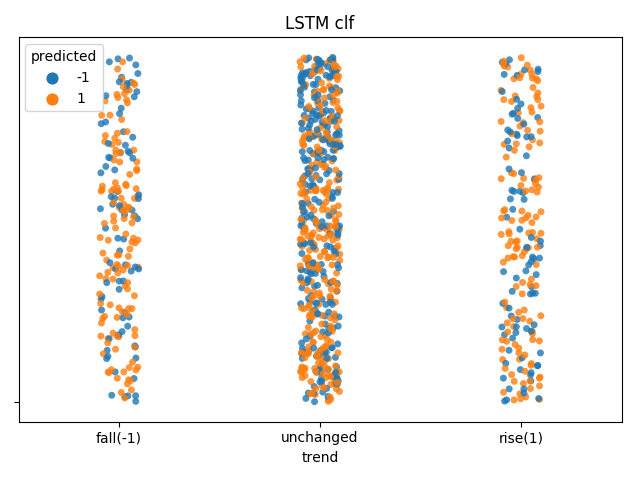
\includegraphics[scale=0.3]{cl_lstm_npd.png}
	\caption{LSTM classifier doesn't perform well} \label{fig 4}
\end{figure}

The evaluation standards we used here are as follows.\\

1. The prediction is correct if and only if true price trend is the same as the predicted one, or true price trend is ‘remaining’. \\
2. The prediction is correct if and only if the first varied (rise or decline, may not be next tick) trend is the same as the predicted trend (next tick).\\

In general, mean square error is one of the most commonly used loss function but there is a deficiency that it cannot distinguish some complicated cases. For instance, \\
\begin{center}
\begin{tabular}{|c|c|c|}
	\hline
	$y_{true}$ & $y_{pred}$ & loss\\
	\hline
	0.02 & -0.01 & 0.0009\\
	\hline
	0.04 & 0.01 & 0.0009\\
	\hline
\end{tabular}
\end{center}

As shown in table, two samples are given the same loss. However, obviously the prediction of first sample is worse since its prediction of trend is totally wrong. Inspired by this observation, we decided to use another improved loss
function defined by
$$
	L(y_{true},y_{pred}) = \frac{\sum_{k}p_k(y_{true}^{(k)} - y_{pred}^{(k)})^2}{N}
$$

where $p_k$ is a punishment coefficient, taking larger value when $y_{true}^{(k)}$ and $y_{pred}^{(k)}$ have contrary signs. 

After several trials we found that the regression of the price of next tick is impracticable, since the price of the current tick, one of our features, will be a strong disturbance. LSTM and other neural networks are very likely to 
learn to ‘follow’ the current price, that is, they will always give a prediction of next tick’s price whose value is almost the same as current price. Therefore, we have to consider other labels to regress. 

A simple idea is to consider the variation of price instead. We can define NPD (next price delta) as the difference of the prices of next tick and current tick, i.e.\\
$$
	\text{NPD} = \text{price of next tick } – \text{ price of current tick}
$$

\begin{figure}[ht]
	\centering
	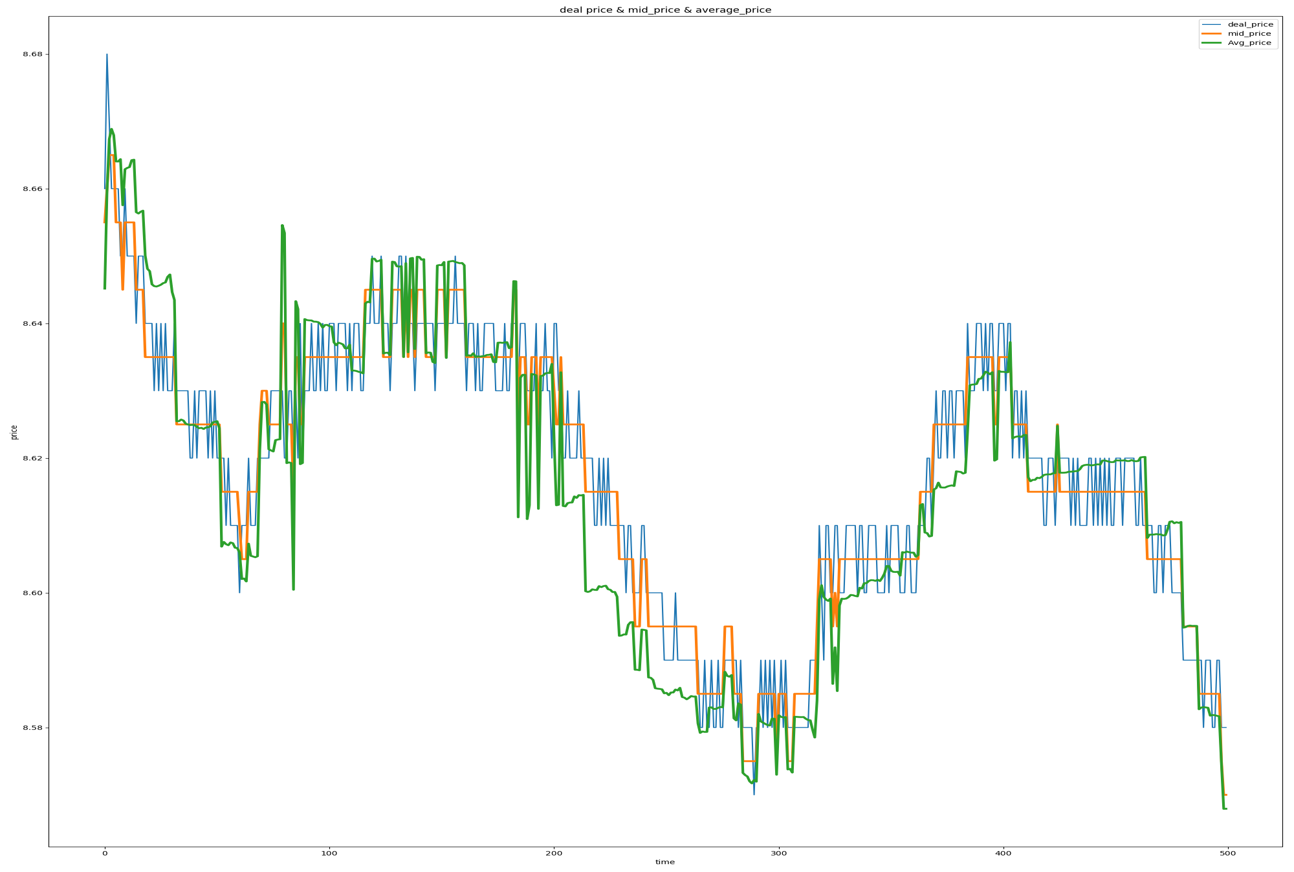
\includegraphics[scale=0.3]{price_mid_avg.png}
	\caption{price \& mid-price \& avg-price} \label{fig 5}
\end{figure}

Mid-price, the mean value of buy1 and sale1 price, is also an important index and has a strong relationship with the true price. Therefore, similarly, the prediction of future mid-price will also be disturbed by the current price, so
we can also define NMPD (next mid-price delta) as the difference of the mid-prices of next tick and current tick, i.e.
$$
	\text{NMPD} = \text{mid-price of next tick } – \text{ mid-price of current tick}
$$

As mentioned above, using regression to predict the trend can preserve more information and hence more effective. However, some regression model like neural networks and boosting are sensitive to imbalanced samples and unfortunately,
NPD and NMPD are both imbalanced. More specifically, over half of the samples are labelled ‘remain unchanged’. This is because in a short period of time there may not be any transaction.\\

\begin{figure}[ht]
	\centering
	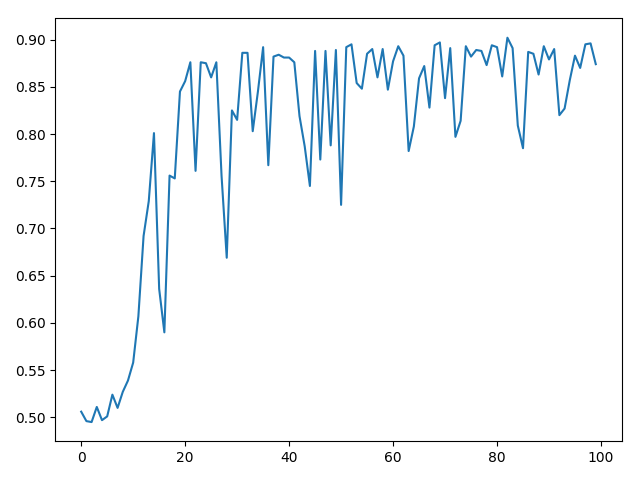
\includegraphics[scale=0.3]{lstm_cl_iter_acc.png}
	\caption{acc - epoch of LSTM} \label{fig 5A}
\end{figure}

\begin{figure}[ht]
	\centering
	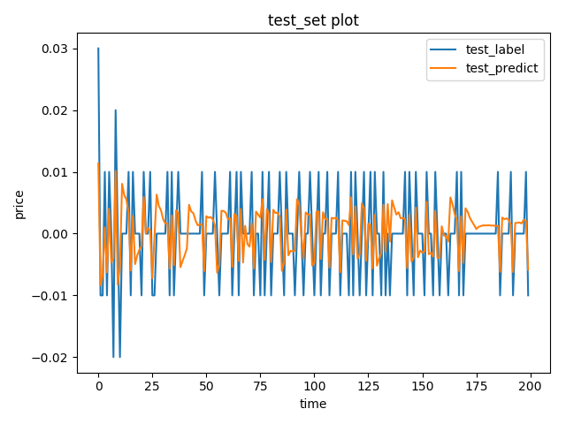
\includegraphics[scale=0.7]{lstm_next_price_delta_local.png}
	\caption{LSTM: next price delta (local)} \label{fig 6A}
\end{figure}

\begin{figure}[ht]
	\centering
	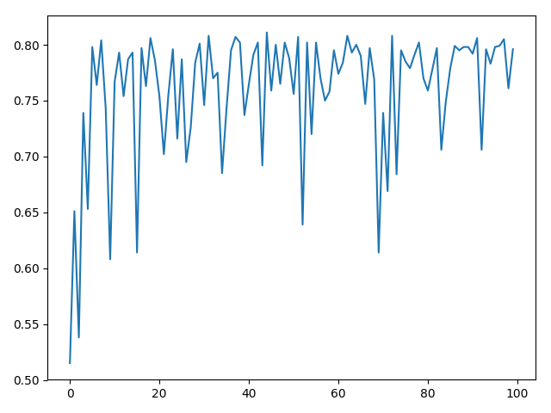
\includegraphics[scale=0.7]{lstm_iter_acc_mid.png}
	\caption{acc - epoch of LSTM} \label{fig 5B}
\end{figure}

\begin{figure}[ht]
	\centering
	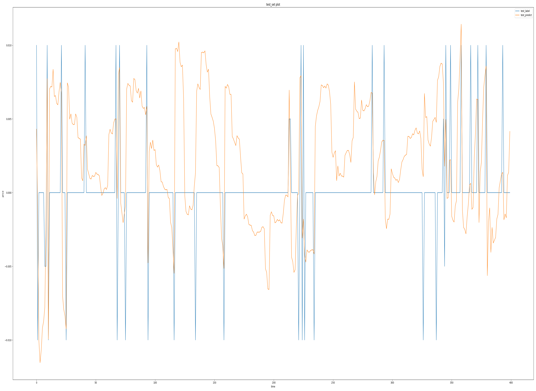
\includegraphics[scale=0.7]{lstm_mid_price_delta_local.png}
	\caption{LSTM: mid price delta (local)} \label{fig 6B}
\end{figure}

%\begin{figure}[ht]
	%\centering
	%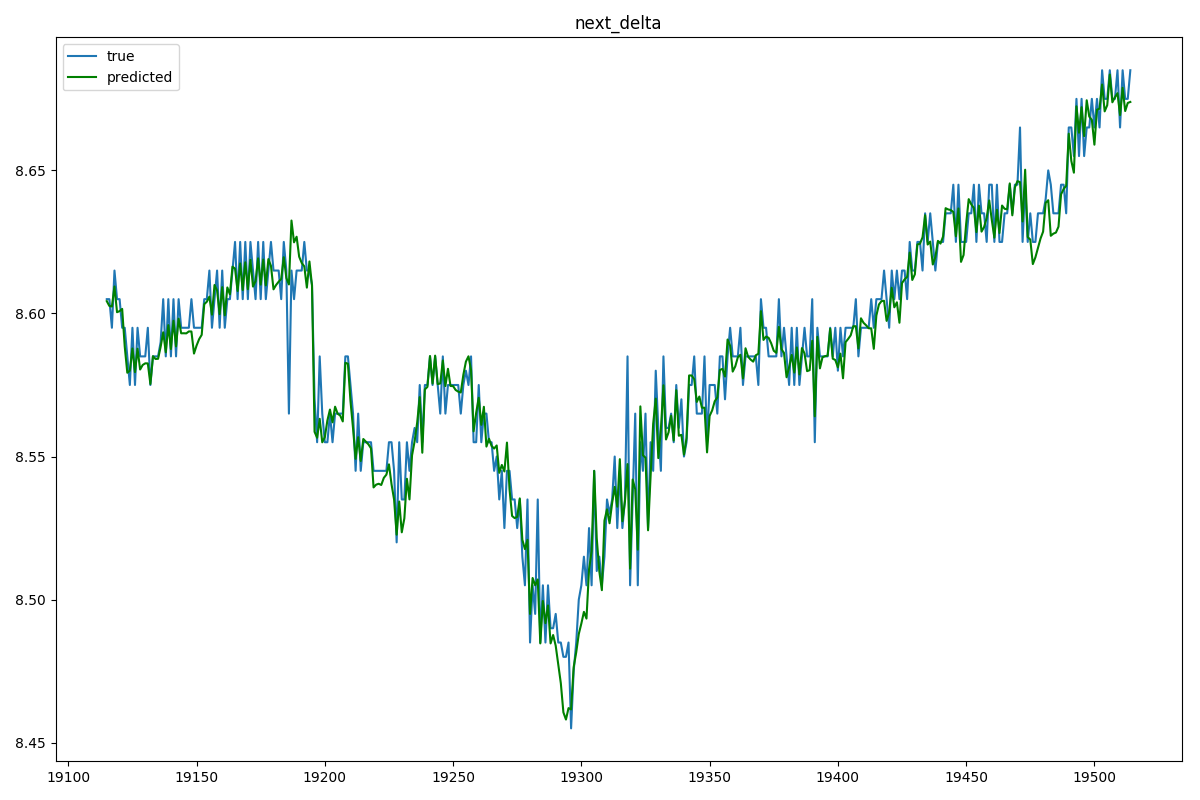
\includegraphics[scale=0.18]{rg_lstm_npd.png}
	%\caption{LSTM: next price} \label{fig 7}
%\end{figure}

%\begin{figure}[ht]
	%\centering
	%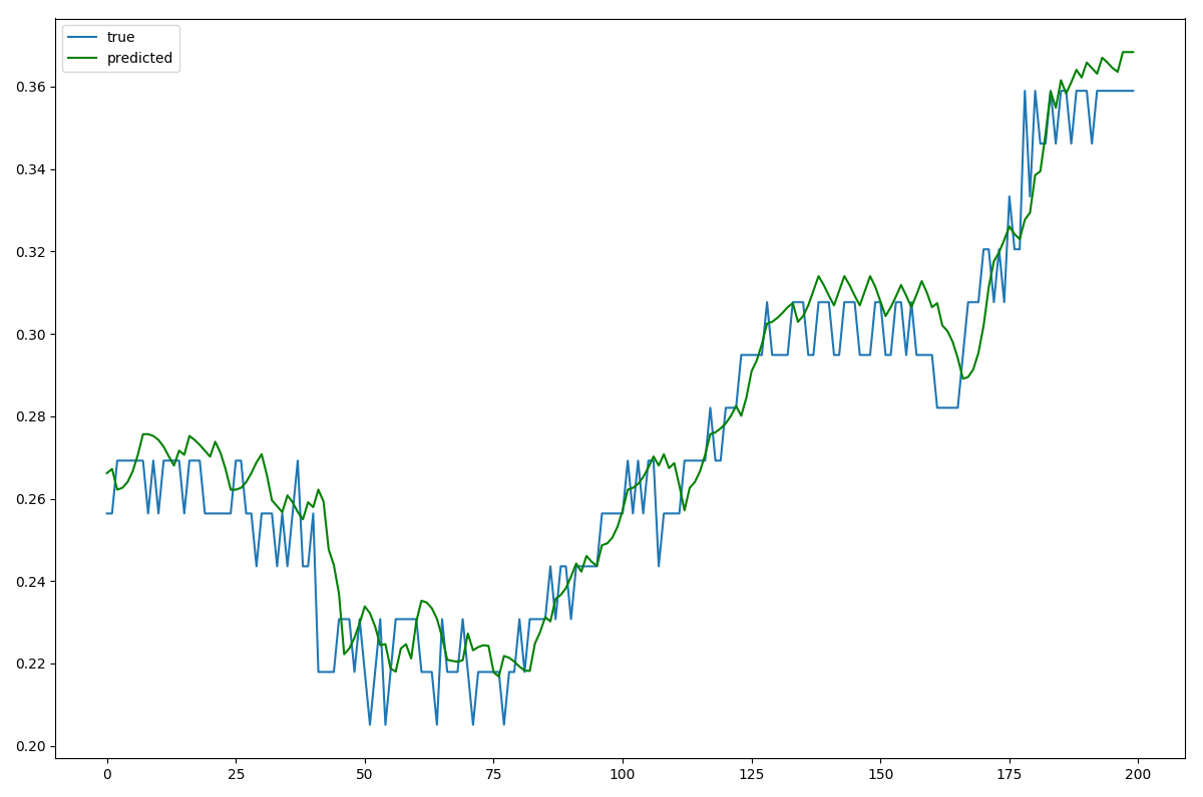
\includegraphics[scale=0.32]{lstm_next_price_local.png}
	%\caption{LSTM: next price (local)} \label{fig 8}
%\end{figure}

The experiments results are as follows.\\

\begin{tabular}{|l|l|l|l|}
	\hline
	& LSTM & XGBoost & Random Forest\\
	\hline
	NPD & 0.920 & 0.909 & 0.906\\
	\hline
	NMPD & 0.817 & 0.801 & 0.824\\
	\hline
	2.5min MPD & 0.741 & 0.712 & 0.709\\
	\hline
\end{tabular}

%\begin{figure}[ht]
	%\centering
	%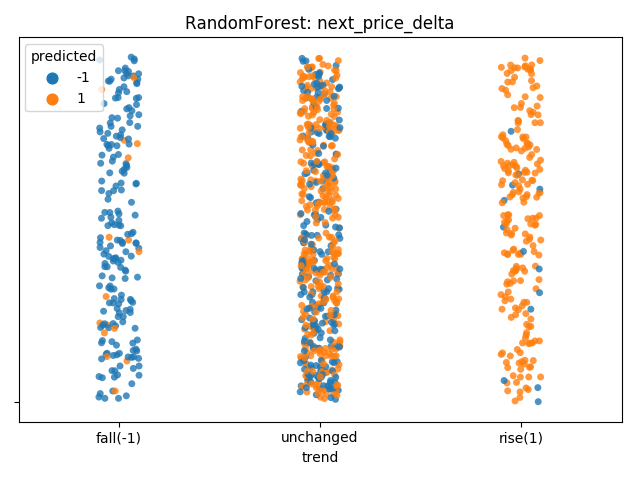
\includegraphics[scale=0.3]{cl_rf_npd.png}
	%\caption{Random Forest classification of next price trend} \label{fig 9}
%\end{figure}

\subsection{Predicting price of a longer period of time}
Although we can predict the price trend of the next tick with a high accuracy rate, such predictions are somewhat short-sighted, and it is difficult to show the trend of stock prices in a broader perspective, which results in
difficulty of applying them in reality. Therefore, we hope to modify our model so that it will have a long-term perspective and predict the price changes in the future for a longer period of time.
\begin{enumerate}
	\item Label construction\\
	If we want our model to learn the rules of price change for a longer period of time, it is necessary to re-examine the label used for supervised learning.To accurately predict the stock price at a certain moment in the future
	seems to be somewhat difficult, so we still use the method of  resolving classification problems by regression. However, in our experiments, the price change trend in 30 seconds has become difficult to predict. In LSTM, even the
	prediction performance in the training set is not guaranteed, let alone the performance on the test set. (p17) However, the poor performance of the LSTM model reveals an important fact that the price of the tick data is stochastic 
	and contains lots of noise since it happens to be the specific transaction price of the last order at the specific moment. Besides, in the problem of predicting the trend of the stock price after 30s, the correlation between the 
	feature and the label is greatly reduced, causing the network to fail to learn the relationship between features and labels on the training set.
	Hence, the priority is to refine this problem by choosing the right method to filter the noise contained in the price out and magnifying the correlation between the existing features and the label. To these ends, we use the
	following formula to generate a new standard:
	$$
		\text{MP}^{(i)} = \frac{\sum_{j=-50}^{49}price^{(i+j)}}{100}
	$$
	As shown in figure, we compare the MP with the stock price and find that the MP reflects the changing trend more nicely, smoothing the stock price fluctuation and simplifying the complexity of the price curve. Accordingly, we define the model's label as:
	$$
		\text{MPD} = \text{MP}_{+2.5min} - \text{MP}_{-2.5min}
	$$
\end{enumerate}

\subsection{Feature Importance}
We utilize a method called Mean Decrease Accuracy (MDA) to calculate feature importance. For each feature, MDA shuffles the values of this 
feature in the test set and then let the model to run the new test set. Then we have a new accuracy. Generally, the lower this new accuracy, 
the more important the corresponding feature.

\begin{figure}[ht]
	\centering
	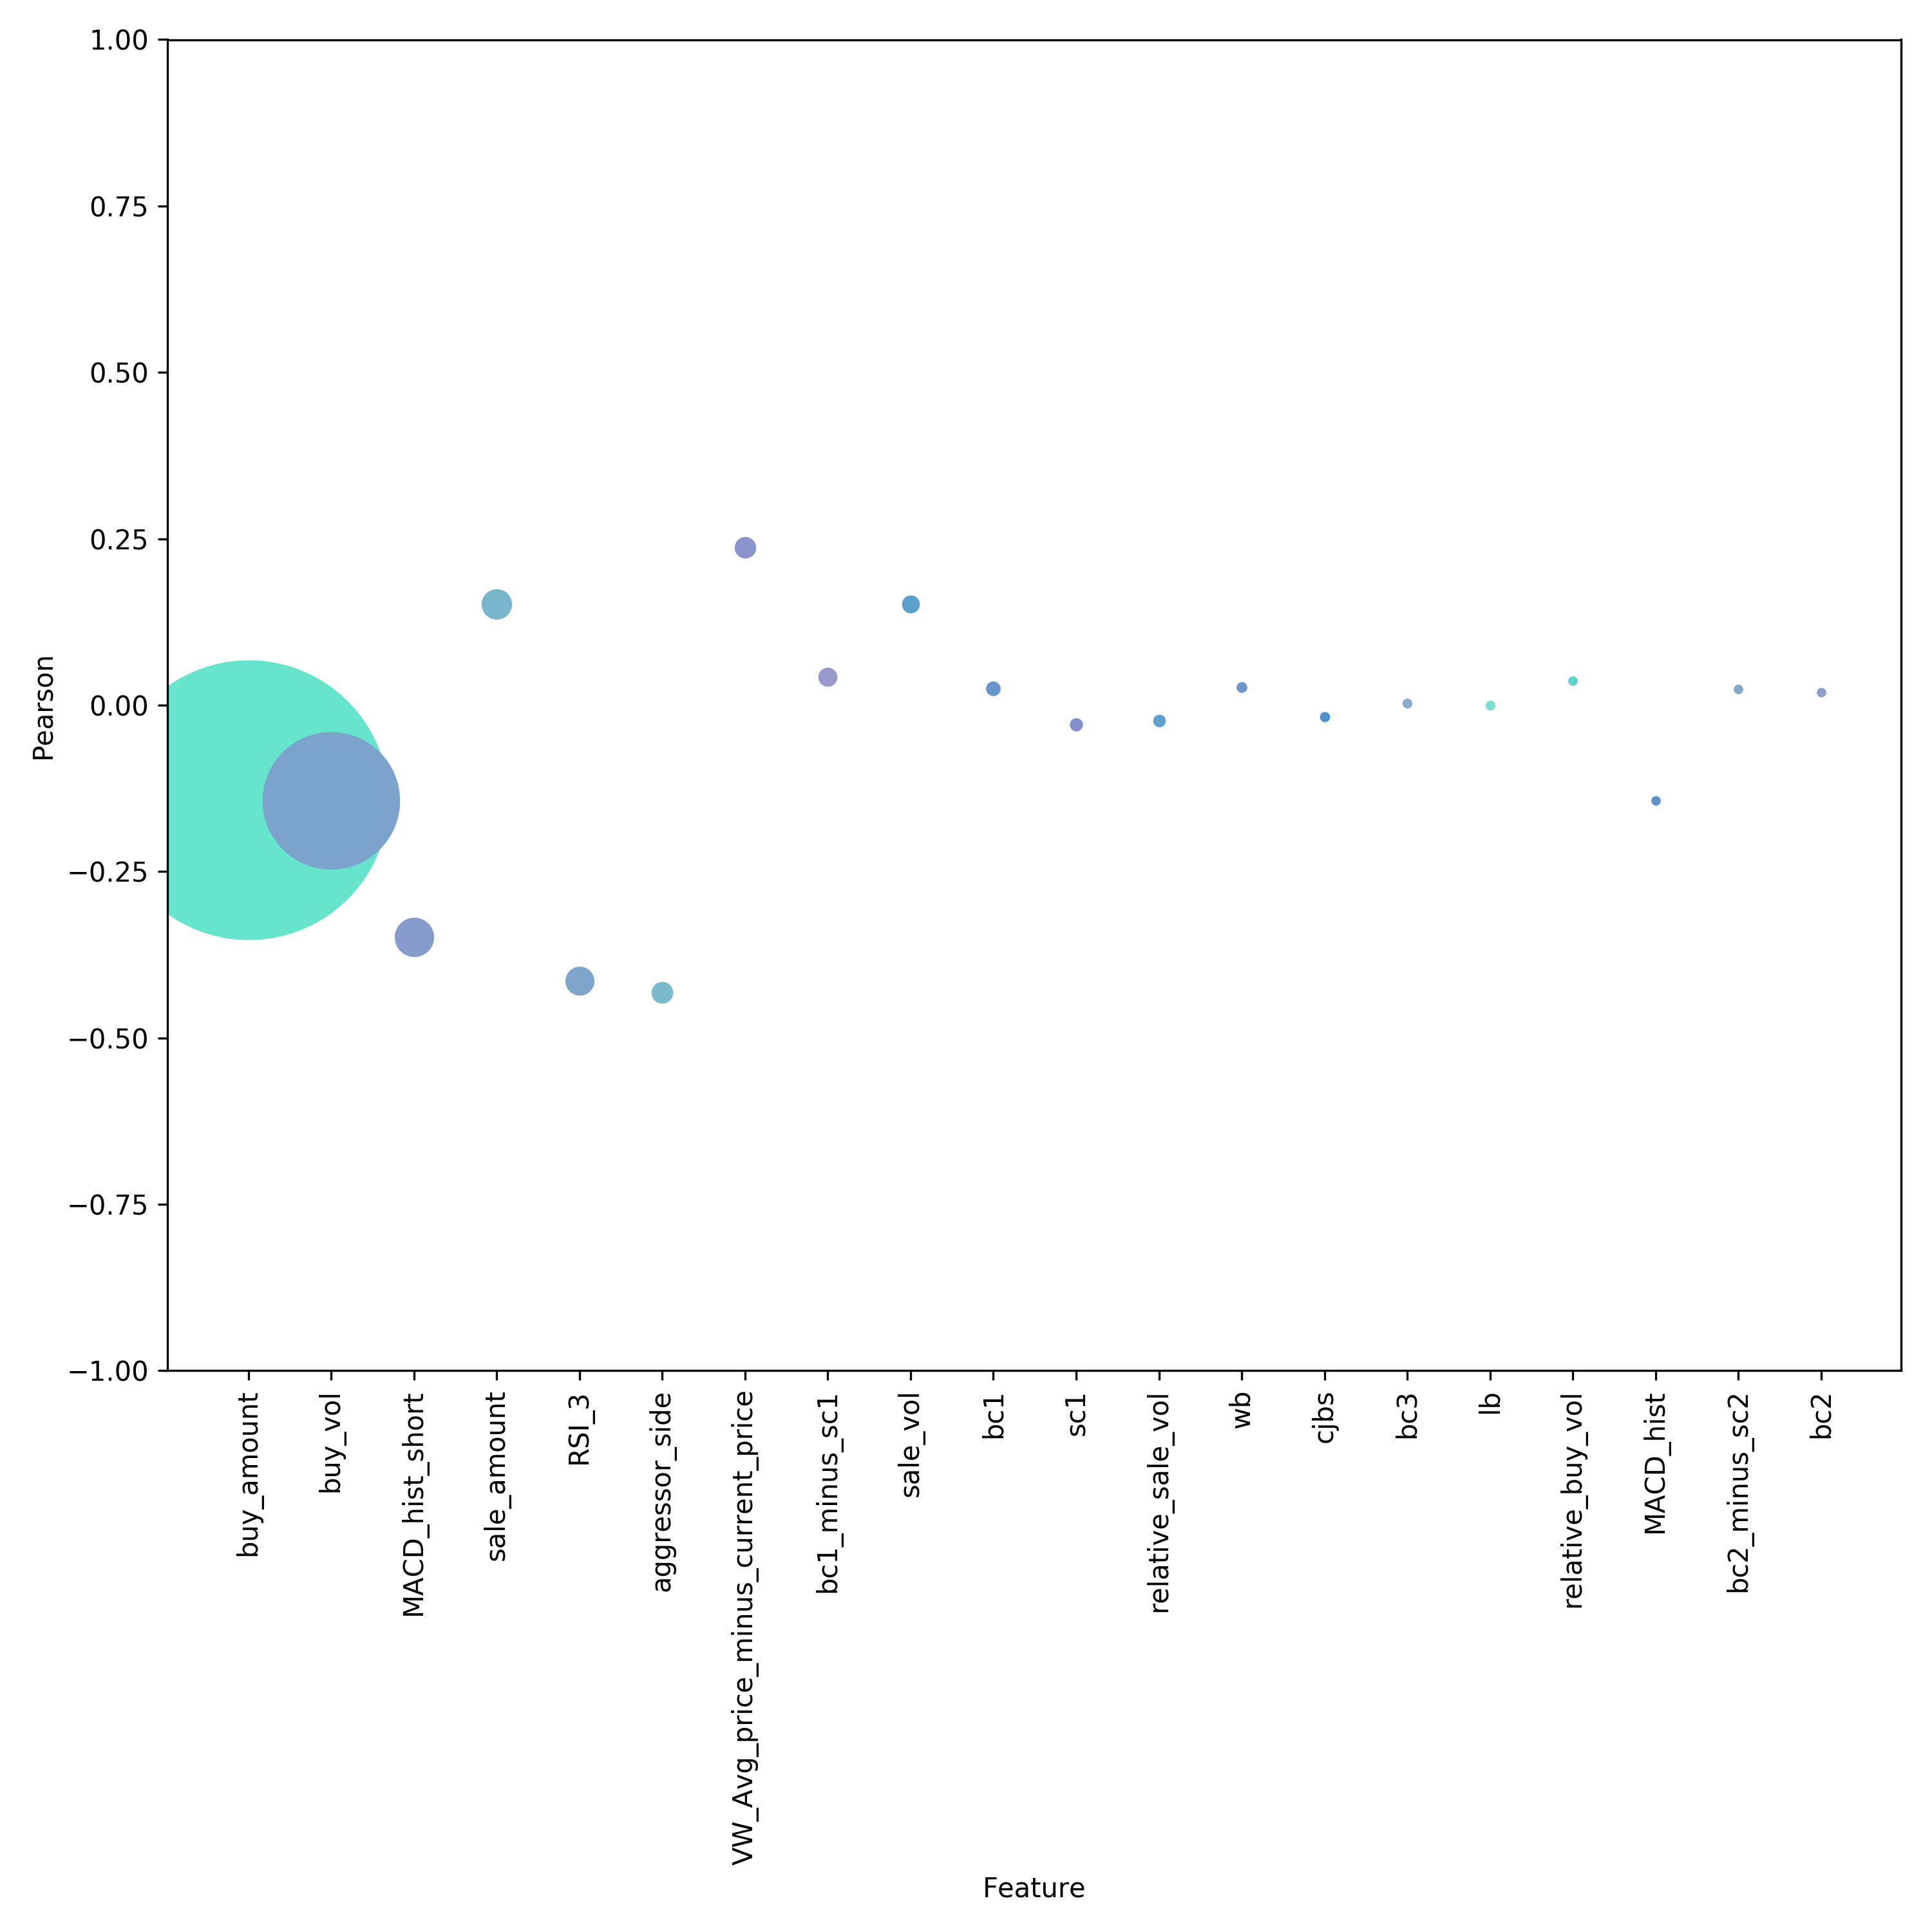
\includegraphics[scale=0.07]{fi_rf_npd.png}
	\caption{Feature importance given by Random Forest} \label{fig 10}
\end{figure}

\begin{figure}[ht]
	\centering
	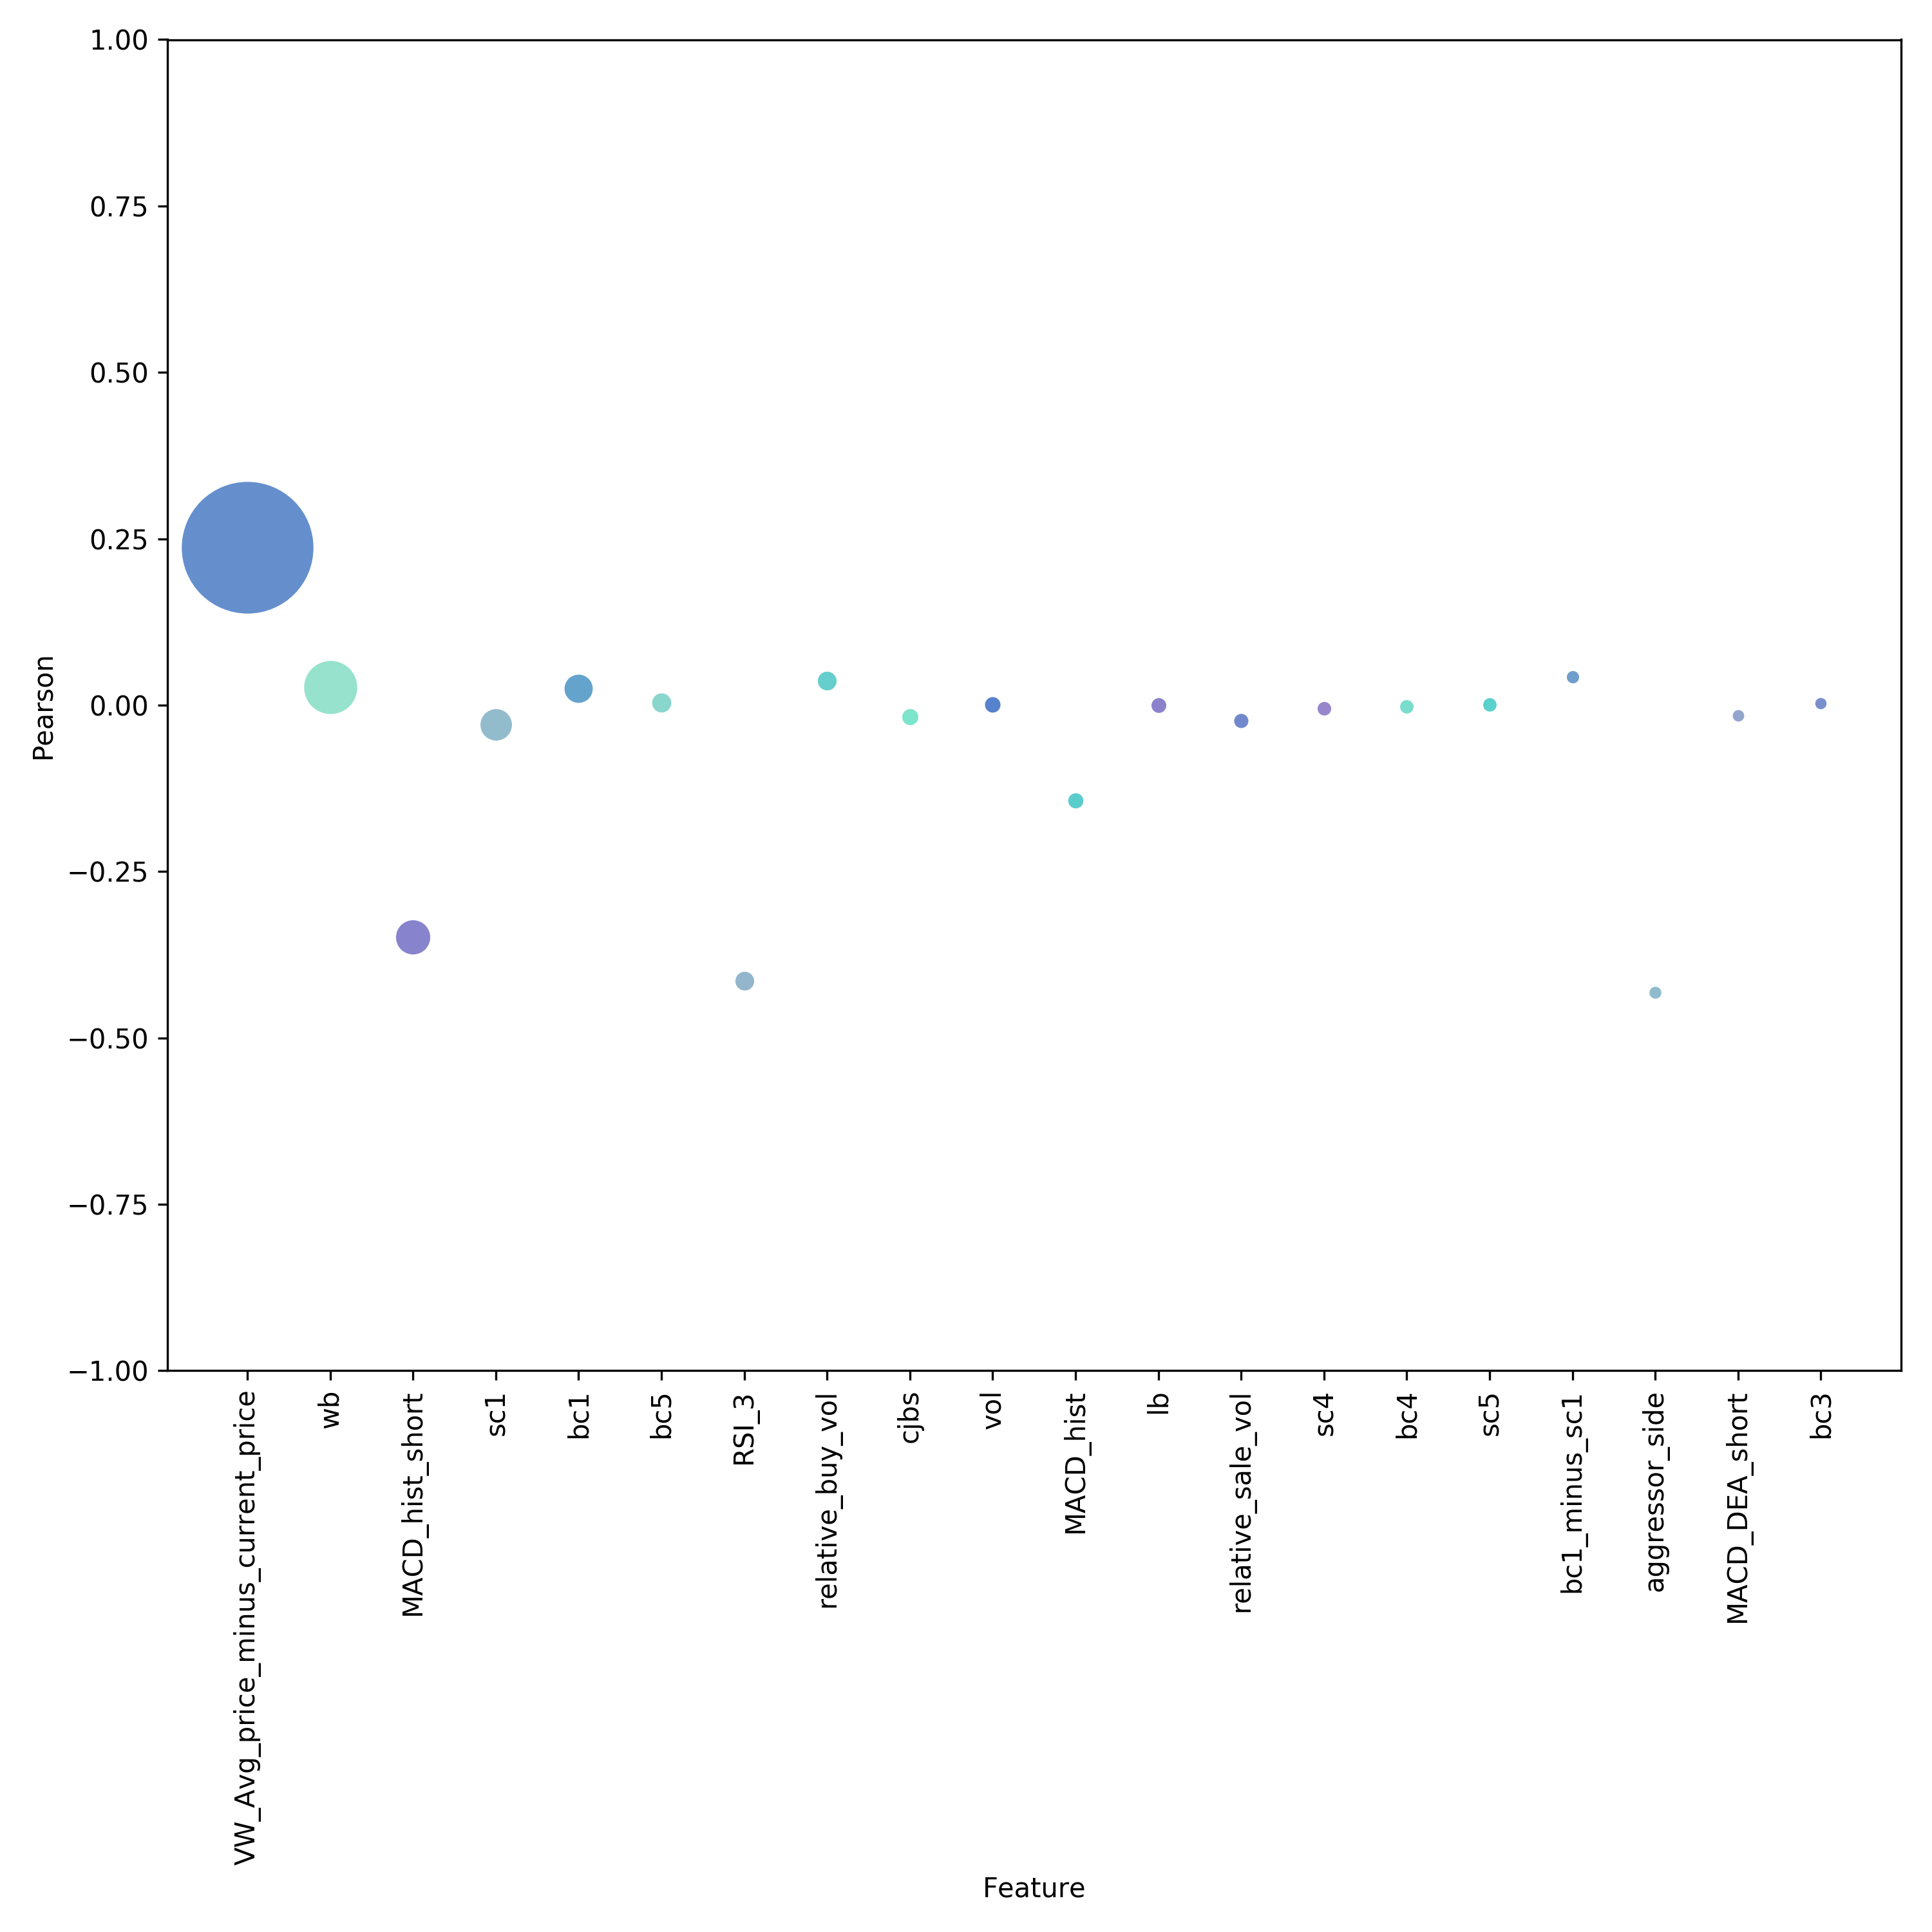
\includegraphics[scale=0.07]{fi_xgboost_npd.png}
	\caption{Feature importance given by XGBoost} \label{fig 11}
\end{figure}

\section{CONCLUSION}
\subsection{Basic hypothesis of stock price}
We assume that the stock price at a certain moment in the future is a statistic that follows a lognormal distribution before it is observed. 
The mean of this lognormal distribution is not fixed, it changes continuously with time. We consider that the outputs of LSTM is something 
close to the change of the mean when learning stock price trend. It is also a continuous variable. But the fact that we have to be aware of 
is the actual stock price is discrete, and the minimum change is 0.01 yuan. Such a unit of change is not small for the stock price change 
under high-frequency environment. In the prediction of the next tick, 96.4\% of the samples have a price change of no more than 0.01 yuan. 
Subsequent analysis will be based on such assumption and fact.

\subsection{Further analysis of experiment results}
\begin{figure}[ht]
	\centering
	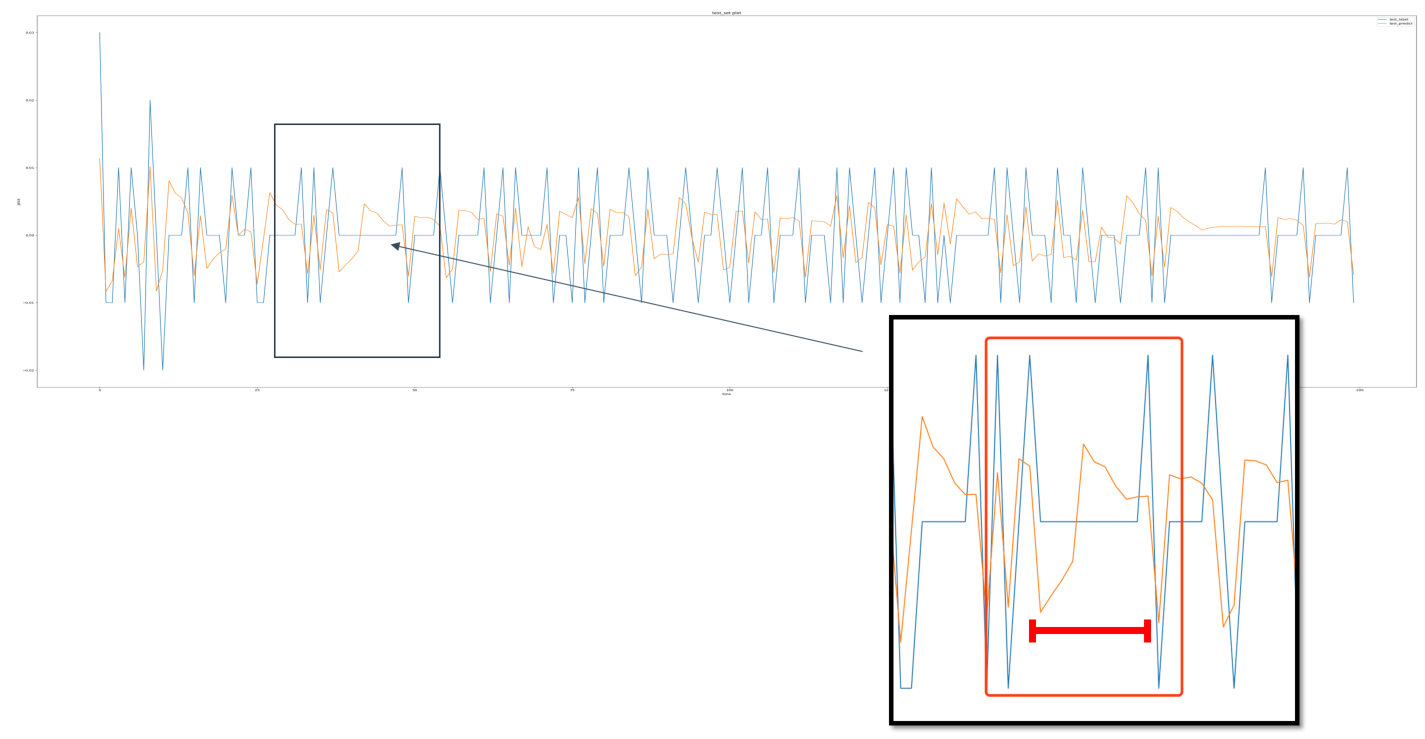
\includegraphics[scale=0.4]{zoom.png}
	\caption{Price delta of both ends of the interval where stock price remains unchanged is 0.01} \label{fig 13}
\end{figure}
As shown in figure 12, the phenomenon that the LSTM prediction value is not zero but the stock price is unchanged is not rare in research on 
price of next tick. Under the assumptions mentioned in the previous section, we think such a phenomenon is reasonable. We consider the output 
of LSTM as the mean of the lognormal distribution mentioned before. The output of LSTM is not zero do not mean that the price of the stock 
will definitely change, only means that stock prices will develop to the price closer to the mean with a higher probability. For example, 
if the output value exceeds 0.005, this means that stock prices have a greater probability of rising. In contrast, If the output value less 
than 0.005 but more than -0.005, this means that stock prices have a greater probability of remaining unchanged. 
Another interesting phenomenon of LSTM’s output is shown in the figure 12. Both ends of the interval that stock price remains unchanged is 
0.01, which means thats stock price has continued to rise during the beginning and end of this time interval. However, the output of the 
network in this interval seems to be unusual. After correctly predicting the rise in stock prices, the output of network drops below zero 
at once, but gradually increases to greater than zero until the stock price changes next time. Under the above analysis, we believe that 
when the output of LSTM does not reach the minimum unit price of 0.01 yuan, the stock price also has the possibility of  change. When this 
change occurred, the stock price is higher than the price expected by the network, so the network will think that the next moment is likely 
to fall, that is the reason why the output of LSTM drops below zero at once . But as time goes by, the expected price difference will 
gradually increase to 0 and continue to grow, until the stock price changes again. Under such  hypothesis, the phenomenon that the stock 
price at high frequencies is often repeated up and down fluctuations can be well explained.

\subsection{Comparison among LSTM, XGBoost and Random Forest}
In most cases LSTM performs better but it requires longer training time and it is more sensitive to hyperparameters. Besides, XGBoost and
Random Forest have stabler performances.

\section{FUTUREWORK}
\begin{enumerate}
	\item Using orderbook data instead of tick-level data based on hypothesis above.
	\item Using LSTM of other structures.
	\item Introducing variance of the stock price distribution.
	\item Ensembling LSTM and XGBoost/Random Forest.
	\item Using Causal CNN.
	\item Generating more practical labels based on trading strategies.
\end{enumerate}

\vspace{0.5cm}

\begin{thebibliography}{1}
\bibitem{IEEEhowto:kopka}
Gers F A, Schmidhuber J, Cummins F. Learning to forget: continual prediction with LSTM[J]. Neural Computation, 2014, 12(10):2451-2471.\label{ref 1}

\bibitem{IEEEhowto:kopka}
Chen T, Guestrin C. XGBoost:A Scalable Tree Boosting System[C]// ACM SIGKDD International Conference on Knowledge Discovery and Data Mining. ACM, 2016:785-794.\label{ref 2}

\end{thebibliography}
\end{document}